% Template for ICASSP-2015 paper; to be used with:
%          spconf.sty  - ICASSP/ICIP LaTeX style file, and
%          IEEEbib.bst - IEEE bibliography style file.
% --------------------------------------------------------------------------
\documentclass{article}
\usepackage{spconf,amsmath,cite}
\usepackage{graphicx}
\usepackage{multirow}
\usepackage{units}
\usepackage{microtype}
\usepackage{paralist}

\newcommand{\secref}[1]{\mbox{Section~\ref{#1}}}
\newcommand{\tabref}[1]{\mbox{Table~\ref{#1}}}
\newcommand{\figref}[1]{\mbox{Figure~\ref{#1}}}
\newcommand{\eqnref}[1]{\mbox{Eqn. (\ref{#1})}}


% Title.
% ------
\title{DRUM TRANSCRIPTION USING PARTIALLY FIXED NON-NEGATIVE MATRIX FACTORIZATION}
%
% Single address.
% ---------------
\name{Chih-Wei Wu, Alexander Lerch}
\address{Georgia Institute of Technology\\
		Center for Music Technology\\
		840 McMillan St. Atlanta GA 30332}

\begin{document}
%\ninept
%
\maketitle
%
\begin{abstract}
A drum transcription algorithm using partially fixed non-negative matrix factorization is presented. The proposed method allows users to separate percussive activities from harmonic activities with pre-trained drum templates and detect drum events from the extracted percussive activation matrix. It is efficient and is robust even with a minimal training set.
A subset from ENST drum data set, which contains single hits and the complete mixtures, has been used for training and testing of the algorithm. 
The system can achieve 56.7 to 78.9\% recognition rate on multiple drums in polyphonic music. 
\end{abstract}
%
\begin{keywords}
NMF, Drum Transcription, Automatic Music Transcription, Music Information Retrieval
\end{keywords}
%
\section{INTRODUCTION}\label{sec:introduction}
Automatic music transcription is one of the most intensively researched areas in Music Information Retrieval (MIR). The reliable extraction of a score (or a score-related representation) from the audio signal will be the core technology of a large number of applications in fields such as music education, systematic musicology, and music visualization. Furthermore, a reliable transcription would enable high-level representations of music signals with the potential of improving virtually any MIR task.

%Transcribing music content into sheet music or any form of score is an essential skill to musicians for analysis and composition purposes. However, It is often considered a time-consuming and non-trivial task, for it requires repetitive listening and integral knowledge of music and instruments. With the advance of computing power and various machine learning techniques, a system that has the abilities to automatically recognize music content has become a plausible idea and interests many researchers in the field of Music Information Retrieval (MIR) \cite{1}. In general, Automatic Music Transcription (AMT) systems could not only serve as a tool to record the music content, identify notes from improvisations, but also lead to the realization of a music intelligence system \cite{2}. To build a complete AMT system, many subtasks and challenges, such as multi-pitch detection, onset detection, instrument recognition, and rhythm extraction, have been attempted [1]. Comparing with pitched instruments, transcribing un-pitched music events such as percussive sounds seem to be less addressed, and a robust algorithm to detect drum sounds in polyphonic music is still an open question in this field.

%WHAT IS CITATION [2]? A: just a reference to make my point on intellegence music system. Removed

A complete transcription system comprises many related sub-tasks such as multi-pitch detection, onset detection, instrument recognition, and rhythm extraction \cite{benetos_automatic_2013}. While the main focus is mostly on pitched instruments, a considerable amount of publications deal with the transcription of percussive sounds in mixture of tonal and percussive instruments. The drum track in popular music conveys information about tempo, rhythm, style, and possibly the structure of a song. A drum transcription system alone enables applications in active listening \cite{yoshii_drumix:_2007}, music education, and interactive music performance \cite{weinberg_interactive_2009}.

%Drum track, especially in pop music, often plays an important role in determining music structure, style, rhythm and tempo. In many cases, it shares the same importance as the harmonic part in the music. That said, a good drum transcription system could provide essential information of the music content, and could potentially facilitate the realization of many interesting applications. For example, a drum transcription and drum source separation task could mutually benefit from each other and provide the possibility to manipulate drum sounds within an existing drum track \cite{3,4}.  Also, music education could be an application of a drum transcription system, for it could help students identify drum event within a polyphonic music, and provide instructions by analyzing and comparing the differences between the input and reference performances. Furthermore, such system could also be integrated as a part of machine listening, improving the existing systems of robotic musicians \cite{5}.

This study explores the application of the popular transcription method of Non-negative Matrix Factorization (NMF) for drum transcription in polyphonic music. The paper is structured as follows: \secref{sec:related works} provides an overview of the research in this area. In \secref{sec:method} we present our approach; evaluation results are being presented and discussed in \secref{sec:Evaluation}. \secref{sec:Conclusion} provides a summary, conclusion, and directions of future work. 

%Therefore, this study aims to explore alternative solutions to drum transcription in polyphonic music. The final goal of this paper is to find a potential direction to push the limit of this task, leading toward further musical applications.
\vspace{-2mm}
\section{RELATED WORKS}\label{sec:related works}

The early attempts to transcribe percussive sounds mainly focused on the classification of signals containing only drum sounds. For these systems, standard approaches with a feature extractor and a subsequent classification engine are able to produce results with high accuracy \cite{%herrera_automatic_2002, 
herrera_automatic_2003}. 
For many real-world applications, however, the input file is a mixture of percussive and harmonic sound sources. Therefore, a drum transcription system is expected to work on this mixture of sounds instead of exclusively on percussive sounds. 
%Therefore, solving this problem in the context of polyphonic music had become another criterion, and different methods could be found in previous research .  
Gillet and Richard divide systems for the drum transcription from mixtures into three categories \cite{gillet_transcription_2008}: (i)~\textit{segment and classify}, (ii)~\textit{separate and detect}, and (iii)~\textit{match and adapt}.  

Systems of the first category (segment and classify) usually segment the audio signal into a series of events by applying automatic onset detection and extract various features from time or spectral domain. Each event segment is then classified based on the extracted features. 
This approach seems to perform well when features are well chosen \cite{gillet_automatic_2004, dittmar_drum_2005}. However, a sufficient amount of training data and carefully adjusted pre-processing is required in order to get good results. Furthermore, the possibility of  simultaneous sounds increases the number of  classes significantly.

The second type of approaches (separate and detect) is based on the assumption that the music signal is a superposition of different sound sources. By decomposing the signal and into source templates with corresponding activation functions, the music content could be transcribed by identifying the templates and analysing the activities for each template. 
Different methods such as Independent Subspace Analysis \cite{fitzgerald_sub-band_2002}, Prior Subspace Analysis \cite{fitzgerald_drum_2003}, and Non-negative Matrix Factorization (NMF, see below) \cite{moreau_drum_2007,alves_drum_2009} fall into this category. The advantage of these approaches is that they usually are easier to interpret since most of the decompositions are done on the spectrogram of the signal. Furthermore, the handling of simultaneous and overlapping events is inherent to the approach. However, in the context of NMF with a pre-determined dictionary matrix, whether or not the templates are representative enough is one potential problem. Another difficulty is the determination of the rank required for the decomposition process. The third type of approaches (match and adapt) uses pre-trained templates to detect drum events \cite{yoshii_drum_2007}. The templates are searched for the closest match and adapted in an iterative process. %In order to cover a wide range of sounds, multiple seed templates need to be prepared prior to the process. I AM NOT SURE IF I UNDERSTOOD PROPERLY --- PLEASE DOUBLECHECK. That sentence is actually from their paper's conclusion.. but I guess I could skip that since I didn't actaully look into details about they methods.
 
%WHAT ABOUT THESE PUBLICATIONS --- THEY ARE NOT REFERENCED IN THE OVERVIEW: \cite{scholler_sparse_2011}. I didn't cite this one
%delete one citation here
In this paper, we proposed a method using partially fixed NMF to transcribe drum events in polyphonic signals. The idea of using NMF with prior knowledge of targeting source within the mixture has been used in source separation tasks \cite{smaragdis_ssnmf_2007}, and multipitch analysis \cite{raczynski_hnmf_2007}. The method described in this paper has similar ideas with these prior works but with different emphasis: 1. The proposed method focuses on a real world scenario that users only have limited amount of training samples that might be different from the targeting source 2. The proposed method uses a small dictionary matrix, which is efficient and easy to interpret for music transcription task.   

\vspace{-2mm}
%maybe describe the partially fixed idea? 
\section{METHOD}\label{sec:method}
\subsection{Algorithm Description}\label{subsec:algorithm description}
% introduce NMF here
%In this paper, we present a method based on NMF. 
Although NMF has been proven to be effective in music transcription \cite{smaragdis_non-negative_2003}, it is still difficult to determine the number of sources in the target signal for a correct rank parameter setting. The goal of our system is the transcription of drum tracks in complex mixtures while only requiring a few drum samples for training prior to the decomposition process. 

The basic concept of NMF is to approximate a matrix $V$ with matrices $W$ and $H$ as $V \approx WH$ with the non-negativity constraints. Given a $m \times n$ matrix $V$, NMF will decompose the matrix into the product of a $m \times r$ matrix $W$ and a $r \times n$ matrix $H$, with $r$ being the rank of the NMF decomposition. $W$ is the dictionary matrix, and $H$ is the activation matrix. In most audio applications, $V$ is the spectrogram to be decomposed, $W$ contains the magnitude spectra of the salient components, and $H$ indicates the activation of these components with respect to time. The matrices $W$ and $H$ are obtained through an iterative process that minimizes a distance measure between the target spectrogram $V$ and its approximation. \cite{lee_algorithms_2000}. 

The application of this method to music transcription, however, offers some challenges. 
First, the number of sound sources and notes within a music recording is usually unknown. It is therefore difficult to estimate a correct rank number and obtain a clear representation of the decomposed  components. 
Second, it is hard to identify the corresponding instrument of every component in the dictionary matrix $W$, especially when the rank is very high or very low. 
Third, when multiple similar entries exist in the dictionary matrix, the corresponding activation matrix could be activated at these entries simultaneously making it harder to interpret the results. %MAYBE THERE IS A POINT TO BE MADE ABOUT THE ACTIVITY MATRIX AS WELL?
Different methods have been proposed in the previous studies to address these issues. Virtanen trained an SVM to separate drum components from the harmonic components; the rank number was derived empirically during the factorization process \cite{helen_separation_2005}. The identified drum components and their corresponding activities could later be used to reconstruct the drum signal, resulting in a system for drum source separation. Virtanen's approach requires a significant amount of training data for the classifier and, more importantly, the results can be expected to be very susceptible to choice of rank. %However, this method requires separated data to train the classifier, and the results could be data-dependent.
%I think I need to be careful in this paragraph... 

Yoo et al.\ proposed a co-factorization algorithm \cite{yoo_nonnegative_2010} to simultaneously factorize a prior drum track and a target signal, and use the basis matrix from the drum track to identify the drum components in the target signal. This method ensures that the drum components in both dictionary matrices remain percussion only over the iterations, and thus proper isolation of the harmonic components from the drum components. Since they focus on drum separation rather than drum transcription, they can work at very high ranks, but the approach is not directly applicable to the transcription problem because of the probable lack of interpretability of the dictionary matrix.
%============= Factorization figure
\begin{figure}
 \centering 
% \centerline{\framebox{
% 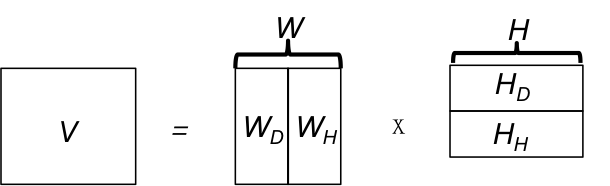
\includegraphics[width=8.5cm]{factorization_small.png}}}
  \centerline{
 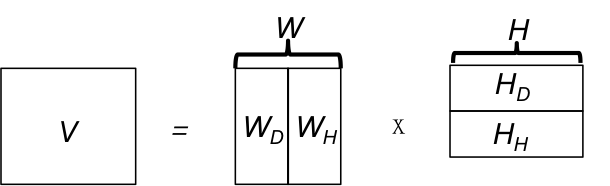
\includegraphics[width=6.5cm]{factorization_small.png}}
 \caption{Illustration of the factorization process. Subscript $D$: drum components $H$: harmonic components.}
 \label{fig:factorization}
\end{figure}
% introduce my modification here 

Nevertheless, their work inspired our approach to drum transcription. \figref{fig:factorization} visualizes the basic concept from the work of Yoo et al.: the matrices $W$ and $H$ are split into the  matrices $W_D$ and $W_H$, and  $H_D$ and $H_H$, respectively. Instead of using co-factorization, however, we propose to initialize the matrix $W_D$ with drum templates and to not modify it during the factorization process. Matrices $W_H$, $H_H$, and $H_D$ are initialized with random numbers. 
The distance measure used in this paper is KL-divergence, in which \(D_{KL}(x \mid y) = x(\log(\frac{x}{y})) + (y - x). \)The cost function as shown in Eq.~\eqref{eq:costFunc} is minimized by applying gradient decent and multiplicative update rules, the matrices  $W_H$, $H_H$, and $H_D$ will be updated according to \mbox{Eqs.~\eqref{eq:updateHD}--\eqref{eq:updateHH}}.  %\eqref{eq:updateHD} \eqref{eq:updateWH} \eqref{eq:updateHH}.  
% equation here
%\begin{equation}
\begin{eqnarray}
\label{eq:costFunc}
J &=& D_{KL}(V \mid W_{D}H_{D} + W_{H}H_{H})\\
%\end{equation}
\label{eq:updateHD}
H_{D} &\leftarrow& H_{D}\frac{W_{D}^T( V / (W_{D}H_{D} + W_{H}H_{H}))}{W_{D}^T}\\
%
\label{eq:updateWH}
W_{H} &\leftarrow& W_{H}\frac{(V/(W_{D}H_{D} + W_{H}H_{H})) H_{H}^T}{H_{H}^T}\\
%
\label{eq:updateHH}
H_{H} &\leftarrow& H_{H}\frac{W_{H}^T (V/(W_{D}H_{D} + W_{H}H_{H}))}{W_{H}^T}
\end{eqnarray}

%\vspace{-5mm}
To summarize, the method described above consists of the following steps:
\begin{inparaenum}
    \item   Construct a $m \times r_D$ dictionary matrix $W_D$, $r_D$ is the number of drum components to be detected.
    \item   Given a pre-defined rank $r_H$, initialize a $m \times r_H$ matrix $W_H$, a $r_D \times n$ matrix $H_D$ and a $r_H \times n$ matrix $H_H$.
    \item   Normalize $W_D$ and $W_H$. 
    \item   Update $H_D$, $W_H$, and $H_H$ using Eqs.~\eqref{eq:updateHD}--\eqref{eq:updateHH}.
    \item   Calculate the cost of current iteration using Eq.~\eqref{eq:costFunc}.
    \item   Repeat step 3 to step 5 until convergence.
\end{inparaenum}

The time positions of the drum events can then be extracted with peak-picking the matrix $H_D$.

\subsection{Implementation}\label{subsec:processing steps}

\figref{fig:flowchart} shows the flow chart of the implemented system. The basic setup is shown on the right hand side. 
The STFT of the signals will be calculated using a window size and a hop size of $2048$ and $512$, respectively. 
A pre-trained dictionary matrix will be constructed from the training set, consisting of isolated drum sounds. 
Next, the partially fixed NMF will be performed with rank $r$ as described above. 
Finally, the activation Matrix $H_D$ is evaluated to determine the onset positions and their corresponding classes.  

\begin{figure}
 \centerline
 \caption{Flowchart of the drum transcription system} %SINCE YOU GIVE OTHER FILTER RESULTS AS WELL: WHY DON'T YOU JUST SAY FILTERING INSTEAD OF REFERRING TO THE HP?
 \label{fig:flowchart}
\end{figure}

%\subsubsection{Template Extraction}\label{subsubsec:template extraction}
As mentioned above, the dictionary matrix $W_D$ is created by extracting a template spectrum from isolated training drum samples. The template magnitude spectrum is median spectrum of all individual events of one drum class in the training set. The length of each event  is approximately \unit[80]{ms}. The templates are extracted for the three classes Hi-Hat (HH), Bass Drum (BD) and Snare Drum (SD).   

%\subsubsection{Activity Detection}\label{subsubsec:activity detection}
High activity values in the activation matrix $H_D$ indicate the presence of a drum event. More specifically, the activity difference of each row of the dictionary matrix could be considered as the onset novelty function of each individual drum. We use a median filter as a standard approach to create an adaptive threshold for peak picking. Heuristically, we set the length and offset coefficient to be \unit[0.1]{s} and 0.12 for every track. 
%I DON'T THINK WE NEED MORE DETAILS HERE --- ESPECIALLY THE EQUATION DOES NOT SEEM NECESSARY.
%The implementation of the median filter is shown in Eq.~\eqref{eq:medianFilter}. The G is the time-varying threshold. Q is a function that extracts the median from previous input signal within a window size = \unit[100]{ms}. Lambda is an offset parameter to control the sensitivity of the threshold.
%% equation here
%\begin{equation}
%G(t) = \lambda + Q(t)
%\label{eq:medianFilter}
%\end{equation}\\
\vspace{-2mm}
\section{EVALUATION}\label{sec:Evaluation}
\subsection{Dataset Description}\label{subsec:data set description}

The experiments have been conducted on the \textit{minus one} subset from the ENST public drum data set \cite{gillet_enst-drums:_2006}. This data set consists of recordings from three different drummers performing on their own drum kits. The set for each drummer contains individual hits, short phrases of drum beats, drum solos, and short excerpts played with the accompaniments. The minus one subset has 64 tracks of polyphonic music, and the sampling rate of every track is \unit[44.1]{kHz} Each track in this subset has a length of approximately \unit[70]{s} with varying style. More specifically, the subset features many drum playing techniques such as ghost notes, flam, and drag; these techniques are considered difficult to identify with existing drum transcription systems. Since we are only interested in the three classes HH, BD, and SD, tracks missing one of these instruments or featuring specific playing techniques have been discarded, leaving a subset of 53 out of 64 tracks.

The accompaniments are mixed with the drum tracks in the data set without any modification (e.g., no level adjustment). The distribution of onset counts per class per drummer is shown in \tabref{tab:onsetCount}. %More details on the creation process of this data set could be found in their corresponding paper.  

%============= Onset event counts in the used tracks
\begin{table}[ht]
\begin{footnotesize}
\centering
\begin{tabular}{|c|c|c|c|c|}
\hline
 & Dr1    & Dr2    & Dr3    & Total \\ \hline
HH        & 1942 & 2145 & 1813 & 5900  \\ \hline
BD        & 2140 & 1488 & 1378 & 5006  \\ \hline
SD        & 2165 & 2079 & 1994 & 6238  \\ \hline
Total     & 6247 & 5712 & 5185 & 17144 \\ \hline
\end{tabular}
 \caption{Onset counts in selected data set}%- IS THIS FOR THE 64 OR THE 53 TRACKS? -- 53!
 \label{tab:onsetCount}
\end{footnotesize}
\end{table}

The drums template have been generated from a different set of tracks in the dataset, which only contains single hits performed by the same group of drummers. Each track contains 5 to 6 single hits on different drums. The onset position of these single hits were determined using the annotated ground truth. 

\subsection{Evaluation Procedure}\label{subsec:evaluation procedure}
We evaluate two different combinations of training and test data: First, we use training samples from all three drummers to train the drum dictionary matrix, and test the system on all $53$ tracks; Second, we investigate cross-performer validation. %as shown in \figref{fig:cross}. 
The training samples are selected only from one drummer, and test on the other drummers' recordings. This scenario should be similar to a real-world use case for which the trained drum sounds are not necessarily similar to the drum sounds in the target signals.

%%============= Cross-performer validation figure
%\begin{figure}
% \centerline{%\framebox{
% 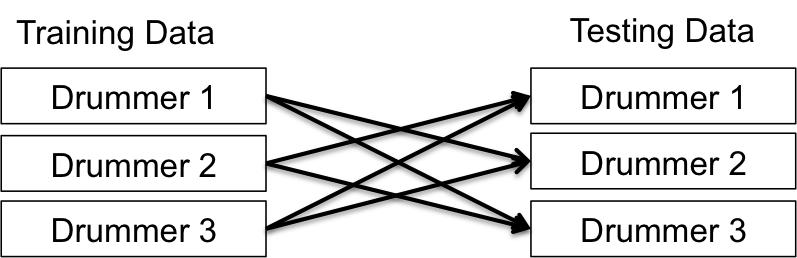
\includegraphics[width=8.5cm]{cross.png}}%}
% \caption{Cross-performer validation process.}
% \label{fig:cross}
%\end{figure}

The evaluation metrics follow by the standard calculation of the precision (P), recall (R), and F-measure (F). % as shown in Eq.~\eqref{eq:precision}, Eq.~\eqref{eq:recall} and Eq.~\eqref{eq:Fmeasure}. The $tp$, $fp$, and $fn$ stand for true positive, false positive, and false negative, respectively. 
An onset is considered to be a match with the ground truth if the time deviation between the annotated and detected onset is less or equal to \unit[50]{ms}.  

\subsection{Evaluation Results}\label{subsec:evaluation results}
In an initial test to determine the rank $r_H$ of the algorithm, $r_H = {5, 10, 20, 40, 80, 160, 320}$ have been tested. The resulting individual F-measures are shown in \figref{fig:rankTest}. A general trend of decreasing performance with increasing $r_H$ can be observed, especially for lower frequency sounds such as SD and BD. Based on this observation, a rank number $r_H = 10$ is chosen in current setup.

%In an initial test to determine the rank $r_H$ of the algorithm, a range of $r_H$ from 5 to 320 have been tested. The results indicates a general trend of decreasing performance with increasing $r_H$. Therefore, in current setup, a rank number $r_H = 10$ is chosen. %SO IS THIS THE OVERALL RANK HERE OR ONLY THE HARMONIC RANK?

%============= Rank Test Figure
\begin{figure}
 \centerline{
 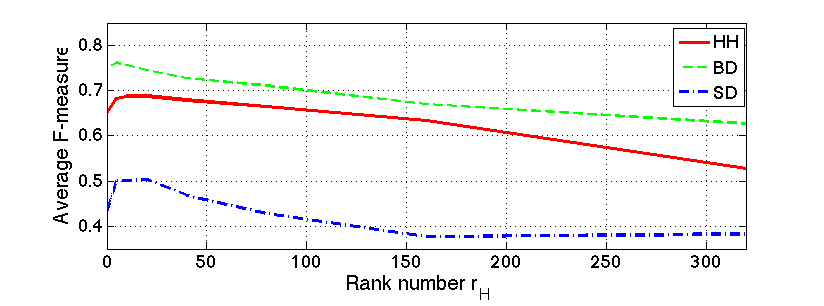
\includegraphics[width=8.5cm]{rankTest.png}}
 \caption{Average F-measure versus harmonic rank $r_{H}$}%WHY NOT ADD A GRID AND MAYBE INCREASE LINE THICKNESS?
 \label{fig:rankTest}
\end{figure}

%\subsubsection{Evaluation I}\label{subsec:Evaluation1}
%============= Train on All templates
\begin{table}[ht]
\begin{footnotesize}
\begin{center}
\begin{tabular}{|c|c|c|c|}
\hline
Training   & \multicolumn{3}{c|}{All}                         \\ \hline
Testing    & \multicolumn{3}{c|}{All}                         \\ \hline
Instrument & HH             & BD             & SD             \\ \hline
P          & 0.681          & 0.755          & 0.634          \\ \hline
R          & 0.727          & 0.827          & 0.513          \\ \hline
F          & \textbf{0.703} & \textbf{0.789} & \textbf{0.567} \\ \hline
\end{tabular}
\end{center}
\caption{Transcription results using all training templates}
\label{tab:basicResults}
\end{footnotesize}
\end{table}
  
\tabref{tab:basicResults} shows the results (precision, recall, and F-measure) when using the complete training and test set.
%It can be observed that using the filters does not necessarily improve the results. The combination of three filters in particular seems to improve results slightly for HH, but the drop in precision of the other classes results in a lower F-measure. In the third, high-pass-only, case we can identify a general trend for improved results in all classes, although the increase for SD and especially BD is rather negligible. These small increase might due the random initialization of the harmonic dictionary, but the deviations are not significant.   
%COMPARE OVERALL RESULTS WITH (THE) OTHER PUBLICATION(S).
Comparing with the reported F-measure of 77.7\%, 65.0\% and 64.8\% for HH, BD and SD in \cite{gillet_transcription_2008}, our results show better performance on BD, but slightly worse performance in SD and HH. However, in our method, the training process require less amount of training data to achieve the results at same level, which could potential provide a better use case for a more generic drum transcription system.     


%The results in the middle column of \tabref{tab:basicResults} indicate that by filtering the templates and signals with constant cutoff frequencies, the performance of BD and SD drop slightly.	Some possible reasons might contribute to this result. First, although the filtering process could suppress contents in the unwanted frequency bins, it also could remove many information that might help to differentiate instruments such as BD and Bass Guitar. Second, in current parameter settings, the band-pass and low-pass filtered signals might only have few bins to represent the spectrum, which might increase the difficulty for the semi-NMF to adapt. Third, when the signals are filtered, the current rank setting $r_H$ might not be optimal for the task.  

%\subsubsection{Evaluation II}
%LETS THINK OF WAYS TO CUMMARIZE THESE THREE TABLES IN ONE TABLE AND A GRAPH, MAYBE DISCARDED PRECISION AND RECALL. MAYBE ALSO OVERALL AVERAGE MEASURES (TRAINING WITH 1, TESTING WITH ALL)?

In order to investigate the dependency of our approach with respect to the similarity of training and test drum sounds, we conduct a cross-performer evaluation as mentioned in \secref{subsec:evaluation procedure}. %No filters have been applied during the process. 
Their results are listed in \tabref{tab:crossResults}.

%============= Cross-Performer results 
\begin{table}[ht]
\begin{footnotesize}
\begin{center}
\begin{tabular}{|c|c|c|c|c|c|}
\hline
\multicolumn{2}{|c|}{Training} & Dr1            & Dr2     & Dr3            & \multirow{2}{*}{Avg.} \\ \cline{1-5}
\multicolumn{2}{|c|}{Testing}  & Dr2+Dr3        & Dr1+Dr3 & Dr1+Dr2        &                       \\ \hline
HH             & P             & 0.661          & 0.662   & 0.660          & 0.661                 \\ \hline
               & R             & 0.747          & 0.719   & 0.726          & 0.731                 \\ \hline
               & F             & \textbf{0.701} & 0.689   & 0.691          & 0.694                 \\ \hline
BD             & P             & 0.811          & 0.641   & 0.859          & 0.770                 \\ \hline
               & R             & 0.905          & 0.742   & 0.915          & 0.854                 \\ \hline
               & F             & 0.855          & 0.687   & \textbf{0.886} & 0.810                 \\ \hline
SD             & P             & 0.724          & 0.543   & 0.727          & 0.665                 \\ \hline
               & R             & 0.538          & 0.429   & 0.539          & 0.502                 \\ \hline
               & F             & 0.617          & 0.479   & \textbf{0.619} & 0.572                 \\ \hline
\end{tabular}
 \caption{Transcription results of cross-performer validation.}
 \label{tab:crossResults}
 \end{center}
\end{footnotesize}
\end{table}

The results show a simple trend: the test set containing drummer 2 give nearly always the best results, regardless of the training set. Also, when training with different drummer's recordings, the F-measure from HH and SD are mostly within the same range as the results reported in \tabref{tab:basicResults} except for BD. This could be due to the fact that Bass Drum of drummer 2 is easy to detect.

These results indicate that this algorithm is relatively robust against differences between the drum template and the sound of the drum to be detected. This would allow to construct a template from different sound sources independent of the recording to be analyzed allowing far more general applications. However, the performance of this setup still needs to be confirmed with a cross-data set validation.

\section{CONCLUSION}\label{sec:Conclusion}

We have presented a drum transcription system for polyphonic music using partially fixed NMF. This method uses a pre-trained dictionary matrix to decompose the target signal and extract the activation matrix. The evaluation results show that this method is able to achieve 56.7 to 78.9\% accuracy for detecting 3 classes in complex mixtures of music. 
The presented method has the following advantages: 
First, the fixed dictionary matrix in the model makes it easier to interpret the corresponding activation matrix for transcription tasks.
Second, simultaneous sounds can be detected separately without the need of training extra classes.  
Third, adjustment of the parameter $r_H$ allows the algorithm to adapt to different different types of polyphonic music. 
Fourth, cross-performer evaluation results indicate a robustness against template mismatches, possibly allowing the application in situations with minimum prior knowledge. 
%Fifth, the approach requires only trivial extensions to be able to be used as a drum separation system as an extension to the current transcription system.
Last but not least, the approach only requires a few drum samples to train the dictionary matrix, and the evaluation results indicate that the performance is comparable with state-of-the art methods at lower algorithmic complexity. 
%FUTURE WORK: ADD HERE WHAT YOU MIGHT WANT TO DO SPECIFICALLY (WHAT YOU PLAN TO DO) AND MORE GENERAL DIRECTIONS.

Possible directions for future work are: 
a comparison between this approach with Probabilistic Latent Component Analysis (PLCA) \cite{smaragdis_plca_2014}. Looking for means to slightly adapt the template during the decomposition might be a way to further generalize the current method. %More generally speaking, we plan to evaluate other distance metrics, cost functions, and adaptation rules in the future. 
Furthermore, automatically estimating $r_H$ for any given signal using probabilistic approach \cite{ouo_inmf_2010} might be a solution to rank selection. Finally, different penalty terms for the cost function, such as sparsity,  temporal continuity \cite{Virtanen_ssnmf_2007} or penalty on the $r_H$ might be taken into account for better adjustment of the current method. To achieve a complete drum transcription system in polyphonic music, however, more factors such as playing techniques and more drum classes still need to be addressed in the future. 




%The text of the paper should contain discussions on how the paper's
%contributions are related to prior work in the field. It is important
%to put new work in  context, to give credit to foundational work, and
%to provide details associated with the previous work that have appeared
%in the literature. This discussion may be a separate, numbered section
%or it may appear elsewhere in the body of the manuscript, but it must
%be present.
%
%You should differentiate what is new and how your work expands on
%or takes a different path from the prior studies. An example might
%read something to the effect: "The work presented here has focused
%on the formulation of the ABC algorithm, which takes advantage of
%non-uniform time-frequency domain analysis of data. The work by
%Smith and Cohen \cite{Lamp86} considers only fixed time-domain analysis and
%the work by Jones et al \cite{C2} takes a different approach based on
%fixed frequency partitioning. While the present study is related
%to recent approaches in time-frequency analysis [3-5], it capitalizes
%on a new feature space, which was not considered in these earlier
%studies."

%\vfill\pagebreak

%\section{REFERENCES}\label{sec:refs}
% -------------------------------------------------------------------------
\bibliographystyle{IEEEbib}
\bibliography{cwIcasspRef}

\end{document}
